The case study was done at Researcher's Night 2015 with two main objectives:
\begin{enumerate}
	\item Cross-validate the findings obtained from a previous experiment~\cite{Angel2017-2}. This experiment was done to study the attribution of different linear and angular velocities, oscillation angel, direction and orientation of the platform to \textit{Anger}, \textit{Happiness}, \textit{Sadness} and \textit{Fear}. A total of 196 were designed, but just 20 treatments were presented to each participant. The questionnaire provided included the four emotions and two mental states (i.e. Excitement and tenderness).
	\item Verify if participants would prefer scenes when the robot expresses emotions or rather moves without any emotion expression. 
\end{enumerate}
To reduce scene variability was used two web-cams and eight Alvar tags to informed a Kalman filter to improve robots localization in the stage. AR tags were detected using the ROS package ar\_track\_alvar~\cite{artag2015}. The distribution of the web-cams and the tags are depicted in Figure~\ref{fig:setup_fourth}. 

\begin{figure}
	\centering
	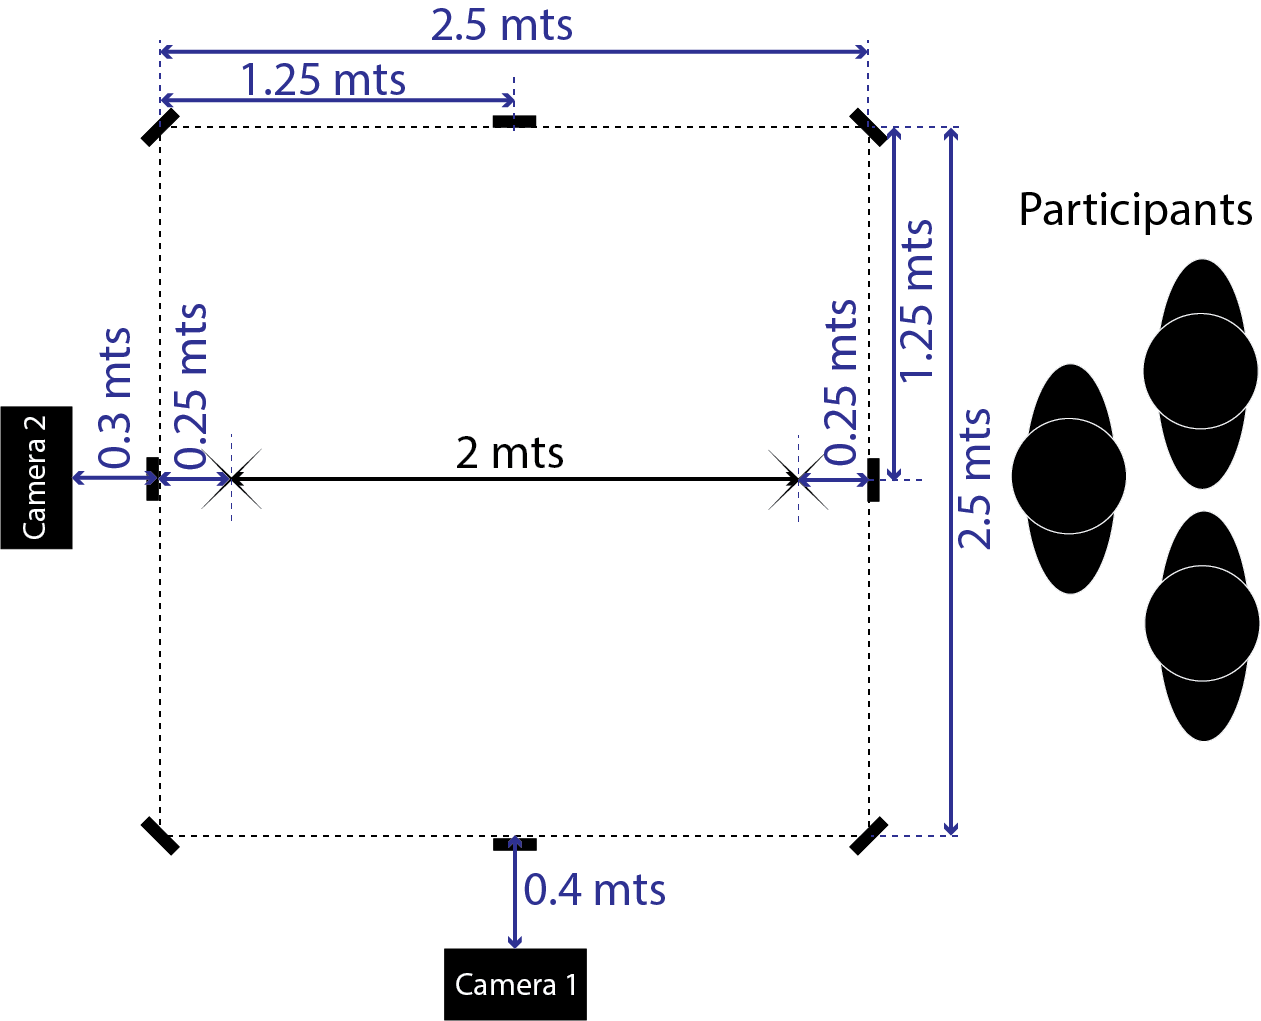
\includegraphics[width=0.45\textwidth]{./Images/FourthCase.png} 
	\caption{Environment setup for the case study. The crosses represent the starting points.}
	\label{fig:setup_fourth}
\end{figure}

\subsection{Emotion Description}

The parameters selected from the experiment to express \textit{Anger}, \textit{Happiness}, \textit{Sadness} and \textit{Fear} are shown in Table~\ref{table:selected_fourth}. As it could be observed, two implementations of each emotions were selected. These implementations were selected considering: (i) the linear velocity should be greater than $0$. In other words the robot should show some linear displacement. And (ii) it should be in the top 10 list of the emotion obtained in the experiment.

\begin{table}
\centering
\small
\caption{Parameters' values selected from the experiment.}
		\label{table:selected_fourth}
		\begin{tabular}{|c|p{0.9 cm}|p{0.9 cm}|p{0.9 cm}|p{1.05 cm}|p{0.9 cm}|}
			\hline
%\rotatebox{90}{\textbf{Emotion } }&
%\rotatebox{90}{\textbf{Direction  ($rad$)}}&
%\rotatebox{90}{\textbf{Orientation ($rad$)} }&
%\rotatebox{90}{\textbf{Linear Velocity ($mm/s$) }}&
%\rotatebox{90}{\textbf{Angular Velocity ($rad/s$) }}&
%\rotatebox{90}{\textbf{Angle ($rad$)}}\\	
\textbf{Emotion}&\textbf{Direc-tion  ($rad$)} & \textbf{Orien-tation ($rad$)} & \textbf{Linear Velocity ($mm/s$) } & \textbf{Angular Velocity ($rad/s$) } & \textbf{Angle ($rad$)} \\
			\hline
			Happiness-1&$0$&$0$&$500$&$3$&$0.349$\\
			\hline
			\co Happiness-2&\co $0$&\co $0$&\co $900$&\co $3$&\co $0.174$\\
			\hline
			Anger-1&$\pi$&$0$&$500$&$3$&$0.087$\\
			\hline
			\co Anger-2&\co $0$&\co $0$&\co $900$&\co $1$&\co $0.087$\\
			\hline
			Fear-1&$\pi$&$\pi$&$900$&$2$&$0.174$\\
			\hline
			\co Fear-2&\co $\pi$&\co $\pi$&\co $500$&\co $2$&\co $0.087$\\
			\hline
			Sadness-1&$\pi$&$0$&$200$&$1$&$0.349$\\
			\hline
			\co Sadness-2&\co $0$&\co $\pi$&\co $200$&\co $1$&\co $0.349$\\
			\hline
			\end{tabular}
\end{table}


\subsection{Scene}

Stage discretization was used to give zones of movements instead of absolute positions. This idea was brought from human theatrical actors, who prepared their movements based on zones on the stage~\cite{wilson2009theatre}. This allows them to adapt their position based on other actors and stage dimensions. Therefore, the stage was discretized in 9x9 matrix as is shown in Figure~\ref{fig:stage_division}. Robot's movements are given in terms of the matrix positions to the Emotional Enrichment System. Robot's final position is calculated by the Emotional Enrichment System during execution. For instance, during the scene's preparation stage was 3 meters per 3 meters, but in the final presentation it was 2.5 meters per 2.5 meters.

\begin{figure}
	\centering
	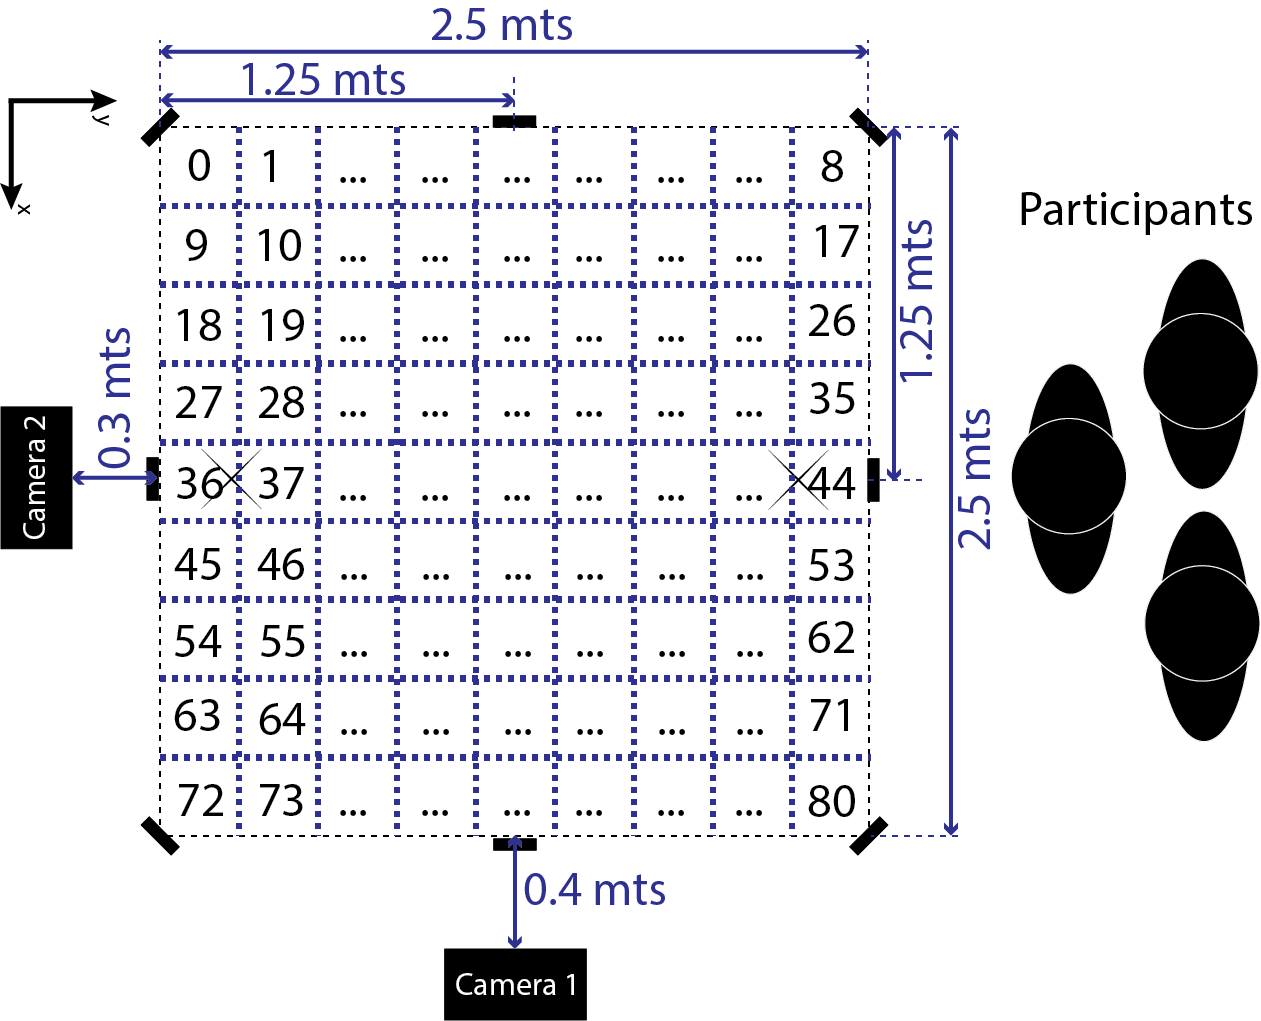
\includegraphics[width=0.45\textwidth]{./Images/FourthCaseScene.png} 
	\caption{Stage discretization  used for the small scene. The blue squares correspond to the each zone, while the numbers correspond to the ID given to each zone.}
	\label{fig:stage_division}
\end{figure} 

Scene's description is the following: the robot starts in the middle of the stage to move to the upstage right (See~\cite{Musical}), close to the right wing. Then, the robot moves to upstage right center and rotates to $\pi/2$ left (See~\cite{Artopia}). Next the robot moves to the right center. Then it goes to the center. When it arrives there, it turns full back and move backwards to downstage center with a full front orientation. There, it turns full back to move to center. Finally the robot turns to profile right and it does a step back; then it goes to the upstage center and then upstage right. The sequence of movements programmed to the robot are depicted in Figure~\ref{fig:movement}.
\begin{figure*}
	\centering
	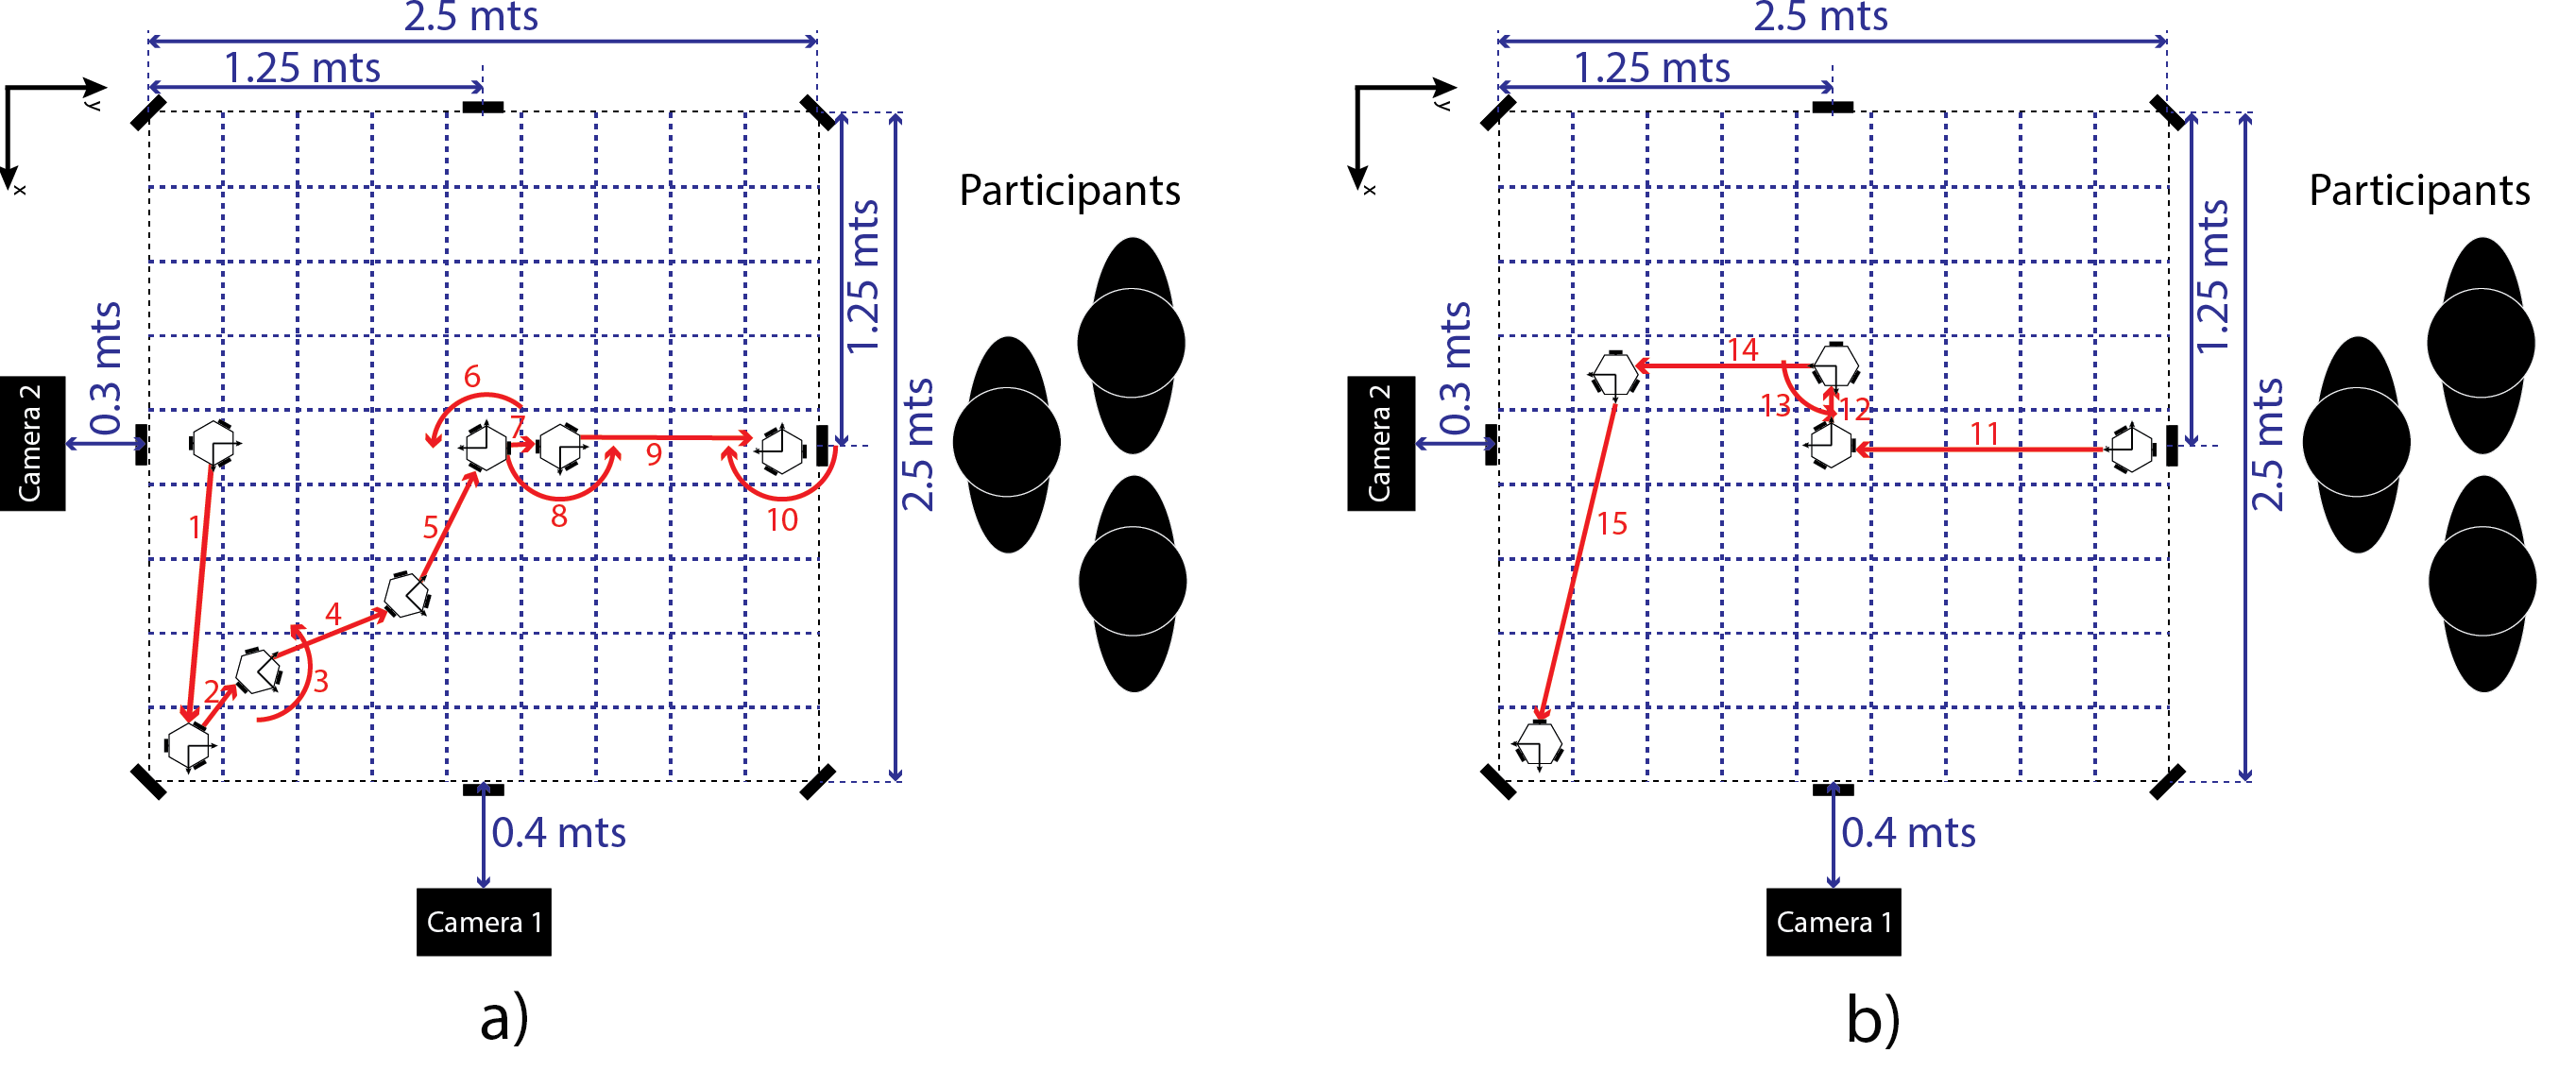
\includegraphics[width=0.95\textwidth]{./Images/fourthCaseSceneD.png} 
	\caption{Sequence of movements provided to the robot. The red arrows show the trajectory, while the numbers show the order among the movements. a) The first ten movements b) The last five movements }
	\label{fig:movement}
\end{figure*}

The relation between emotion and movement is as follow: movements one to five do not express any emotion. Movements six to ten show fear. Movement eleven depicts happiness, and the remaining movements depict sadness. The actions describing this scene are executed by the Emotional Enrichment System and the emotion selection is done manually via a graphical interface.

\subsection{Study}

This case study was done during Researchers' Night, 2015. During a period of two days, people were asked to participate to this study, which was divided in to parts. In the first one, each subject was exposed to two rounds of emotions. The emotion presented and the order were generated randomly before hand. In the second part, they were explained that a small scene was going to be presented twice. Thus, they should to selected the one they like it more. The order of the scenes (e.g. with or without emotion) were generated beforehand. The total number of volunteers was 256: 128 males, 126 females, and 2 that chose not to specify their gender. The average age was 27.29 years, with standard deviation of 16.58, minimum age was 4 and maximum 76.
